\chapter{Fundamentals and Related Work}
\label{chap:fundamentals}

This chapter introduces the reader to the L4 operating system and the \llinux
kernel that runs on top of it. The concept of operating systems noise is
presented along with the \llinux decoupling mechanism which has been designed
to combat this. Then, the fundamentals of how system calls are invoked are
explained, together with the added overhead incurred by the decoupling
mechanism. Finally, some known techniques for reducing system call performance
overhead presented in related work are discussed.

\section{The L4 Operating System}

Originally L4 was developed by Jochen Liedtke as a microkernel-based operating
system of high performance \cite{l4}\cite{l4_performance}. However, nowadays
the name L4 does not refer to a single operating system, but a family of
operating systems or operating system kernels. The L4 application binary
interface has been re-implemented by operating system teams in different
universities such as TU Dresden, Karlsruhe Institute of Technology, and the
University of New South Wales. These implementations added their own
characteristics to the microkernel as well. L4 does not aim to be Unix-like or
POSIX compatible, however some compatibility layers are provided.

\subsection{Fiasco.OC and L4Re}

\emph{L4Re} is the L4 implementation developed at TU Dresden and written in
C++. The operating system is focused on security and performance and it offers
real-time scheduling support with hard priorities. \emph{Fiasco.OC}
\cite{fiasco} is the name of the microkernel itself, which together with the
set of libraries and user-level components that run on top of it, forms the
\emph{L4 Runtime Environment (L4Re)}. Fiasco.OC is also simply called Fiasco,
even though nowadays it is officially referred to as \emph{The L4Re
Microkernel}. These three names will be used interchangeably throughout this
text.

As a microkernel, Fiasco aims to provide user-space programmers with a minimal
interface for essential functionality. Specifically, the user can create
address spaces and threads and it can assign address spaces to threads in order
for programs to be executed. Additionally, the microkernel offers an
inter-process communication (IPC) mechanism that tasks can use in order to talk
to each other. Finally, Fiasco implements thread scheduling in-kernel too.
This contradicts the microkernel philosophy that says that scheduling is a
policy and scheduling implementations shall not be provided by the microkernel
itself, however no efficient alternative has been developed as yet.

Other policies such as memory management are implemented in L4Re but run
completely in user-space (they are not part of the microkernel codebase). The
user-space part of L4Re also provides the infrastructure for loading
applications and offers other system services, thus when combined with Fiasco
it makes for a complete operating system. Development of Fiasco.OC and L4Re is
tightly coupled and happens in parallel.

Fiasco.OC supports symmetric multi-processing (SMP), enabling parallel code
execution in multi-processor systems. The microkernel does not migrate threads
to different cores automatically, but thread migration is possible if
explicitly requested. Fiasco is scalable and suitable for a wide range of
systems, from small embedded devices to large and complex high-performance
computing (HPC) environments.

\subsection{\llinux}

\llinux \cite{l4linux}\cite{l4_performance} is a variant of the Linux kernel
that runs para-virtualized on top of the Fiasco microkernel. Contrary to full
virtualization, para-virtualization is a technique that requires modification
of the guest operating system which then runs while being aware that it is
virtualized.  Fiasco in that case acts as a hypervisor and \llinux can be
characterized as a user-space server in microkernel parlance. \llinux is
modified to the extent that it can run para-virtualized, but these
modifications are kept to a minimum and \llinux remains binary compatible with
the mainline Linux kernel. At the time of writing, \llinux supports the x86,
x86\_64, arm, and arm64 architectures.

The purpose of running a Linux kernel on top of L4 is to reuse legacy code.
The Linux environment includes an enormous collection of drivers, libraries,
and other services that L4 tasks would like to use. However, implementing them
again just for use in L4 would be very expensive and difficult. \llinux can run
unmodified Linux programs as L4 tasks. Additionally, it is possible to write
and run programs that use both Linux and L4 services, by issuing system calls
for both kernels.

In order to achieve this para-virtualization Fiasco employes a scheme that uses
\emph{virtual CPUs} or \emph{vCPUs} \cite{vcpus}. vCPUs are simply L4 threads
that are interruptible. Any L4 thread can act as a vCPU and vCPUs appear to
\llinux as real, physical CPU cores. \llinux uses these vCPUs to multiplex the
execution of its tasks and it performs context switches by binding different
address spaces to the vCPU.

Scheduling works as follows. The Fiasco microkernel manages all physical CPUs
and is responsible for scheduling L4 threads on them. Some of these L4 threads
can be vCPUs. The Linux scheduler on the other hand is responsible for
scheduling Linux processes and it does so on the vCPUs which are assigned to
it. This is depicted in Figure \ref{fig:decoupling} (a). In this example,
Fiasco manages 4 physical CPUs and runs a vCPU thread on the first 3 of them.
These 3 vCPUs are visible to \llinux which can use them for scheduling work as
it sees fit. \llinux cannot interfere with Fiasco's scheduling and vice versa.

\section{Operating System Noise}

Operating system noise or jitter is the overhead introduced by the operating
system when it interrupts the progress of a running application. This overhead
is normally caused by handling interrupts, by maintenance activities of the
kernel such as page reclamation and internal synchronization, and also by
preemption of the user application in order to schedule system daemons.

Operating system noise can be especially problematic on large high-performance
computing (HPC) systems with multiple cores running parallel applications. In
these systems delays introduced on a single CPU core can greatly reduce the
overall performance of the system. Previous studies have shown that as the
number of CPU cores increases, this performance overhead becomes more and more
significant \cite{os_noise1}\cite{os_noise2}\cite{os_noise3}.

On the other hand, lightweight microkernels such as Fiasco, introduce minimal
to no operating system noise at all. Fiasco can be configured in such a way
that if only one thread runs on a core, even periodic timers interrupts are not
delivered to that core. This is ideal for latency-critical applications.
However, when running Linux applications on top of L4, it is the \llinux kernel
which introduces the unwanted execution jitter.

\section{Decoupling Thread Execution from \llinux}
\label{sec:decoupling}

One solution that has been recently proposed and implemented for combatting OS
noise on an L4 environment is decoupling thread execution from the noisy
\llinux kernel \cite{decoupling}.

The main idea behind the decoupling mechanism is to separate the execution of a
thread in a Linux process from the vCPU it is normally running on. This
decoupled thread can then run directly as a standalone L4 thread on a physical
CPU different than the one that executes the vCPU thread. The result of this
separation is that now \llinux cannot preempt this thread interrupting its
progress.

The way this mechanism works is by creating a new native L4 thread that runs in
the same address space as the thread to be decoupled. The execution of the new
thread is then moved to a different CPU, outside the control of the Linux
scheduler. This new thread runs only user-space code for that process and it
can keep executing uninterrupted as it is now managed by the Fiasco
microkernel. We can refer to this thread as the \emph{user thread}.

\begin{figure}[h]
\centering
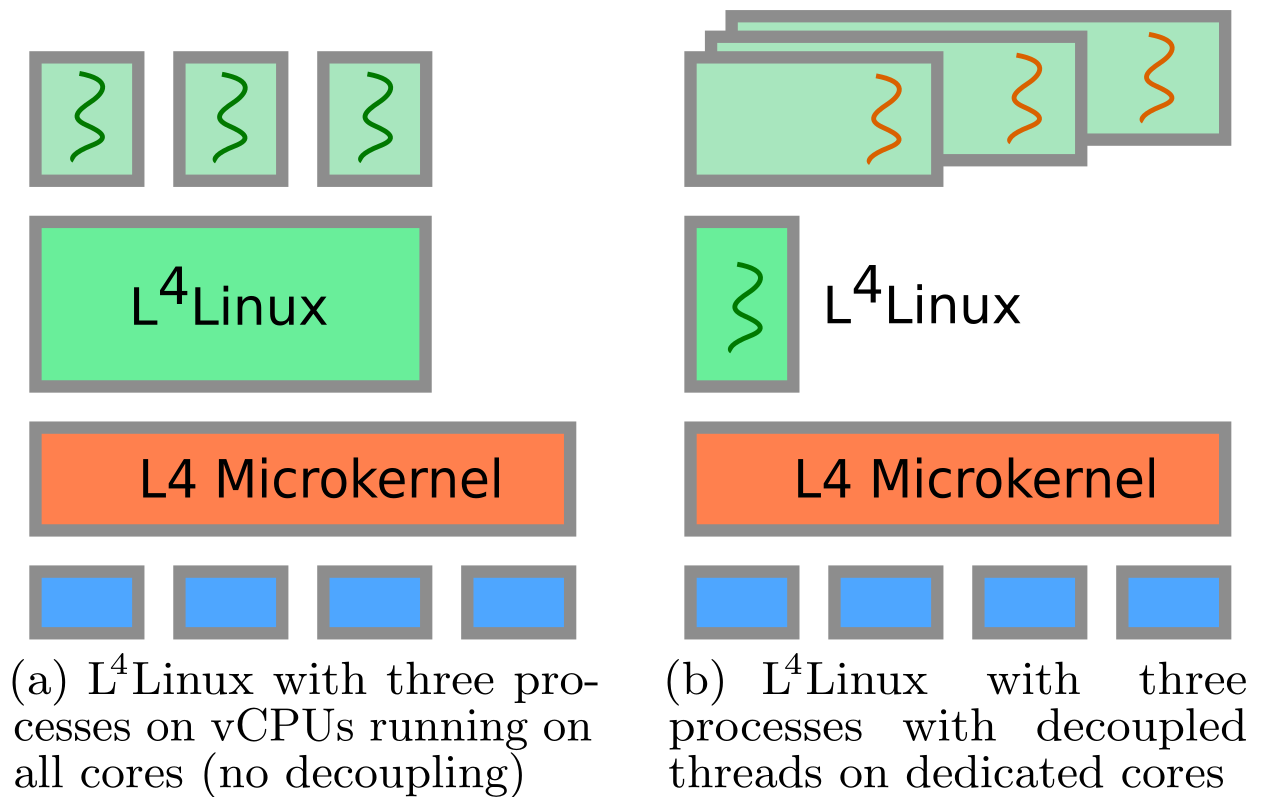
\includegraphics[scale=0.25]{decoupling}
\caption{Illustration of \llinux tasks running in standard and decoupled mode.
         Reprinted from \cite{decoupling}.}
\label{fig:decoupling}
\end{figure}

The original Linux thread remains under \llinux's control, bound to one of its
vCPUs, but it now executes kernel code only. This thread is put to sleep in
order to ensure that the Linux scheduler won't pick it up for execution.  It
only wakes up and gets scheduled when the decoupled, user thread requests Linux
services such as the execution of a \llinux system call or when it generates
any kind of exceptions. After servicing the request, it goes back to sleep
until the user thread generates an exception again. We can refer to this thread
as the corresponding \emph{kernel-side context}.

Using the decoupling mechanism, we can employ a configuration where the
execution of the \llinux kernel is isolated to a small subset of the total
available physical CPU cores. For example, in a system with 32 available CPU
cores, we can have 1 or 2 vCPU threads (bound to 1 or 2 physical CPUs
correspondingly) running \llinux code. The remaining physical CPUs of the
system can be used for running decoupled Linux threads or other native L4
tasks. When the decoupled threads require any services from the \llinux kernel,
such as system call execution or page fault handling, these requests are
forwarded to the appropriate core running \llinux. A similar scenario with 4
real CPUs and 1 vCPU is depicted in Figure \ref{fig:decoupling} (b).

One side effect of this approach, if we take the microkernel out of the
picture, is that it results in a deployment with dedicated user and kernel
CPUs. Even though Fiasco still manages all the cores, it can be configured in a
way that it doesn't interfere with the execution of user processes at all. And
as previously mentioned, studies have shown that having dedicated user and
kernel CPUs can result in significant performance gains \cite{dedicated_cpus}.

Nonetheless, since the new decoupled thread and the corresponding
kernel-context thread are bound to different physical cores, there are certain
forwarding costs associated with the decoupling scheme. Eliminating this extra
overhead, which is explained in detail in the following sections, served as the
main motivation for the work in this thesis.

\section{How System Calls Are Invoked}

System calls are the way with which user programs can request services from the
underlying operating system. They serve as an interface to the kernel which
executes certain code on behalf of user processes. User-space programs can
request hardware services, such as reading from or writing to a disk,
communication with other processes, system information, and various other types
of services. Some examples of Linux system calls are \emph{open}, \emph{read},
\emph{write}, and \emph{fork}. Each operating system offers its own set of
system calls.

\subsection{System Call Invocation on Non-Virtualized Linux}

Most CPU architectures support different CPU modes of different privilege
levels. Usually, user applications execute with the CPU operating on a less
privileged mode (referred to as user mode), while all kernel code executes on
the most privileged CPU mode (referred to as kernel mode). On less privileged
modes, certain hardware instructions will fail or they will behave differently.
This is done for security reasons in order to ensure that user applications
cannot do arbitrary things such as controlling the hardware for malicious
purposes.

Since user programs cannot perform certain actions, they have to ask the
operating system to do it on their behalf. In order for this to happen, there
needs to be a transition from user mode to kernel mode. The CPU will
automatically switch to kernel mode when certain things happen, for example
when a page fault is generated, when an interrupt is received or when there has
been an attempt to execute an illegal instruction. In any of the above cases,
the CPU automatically switches its mode of operation and starts executing the
kernel on a defined entry point. When the kernel wishes to return back to user
mode, it can directly do that using a certain hardware instruction.

\begin{figure}[h]
\centering
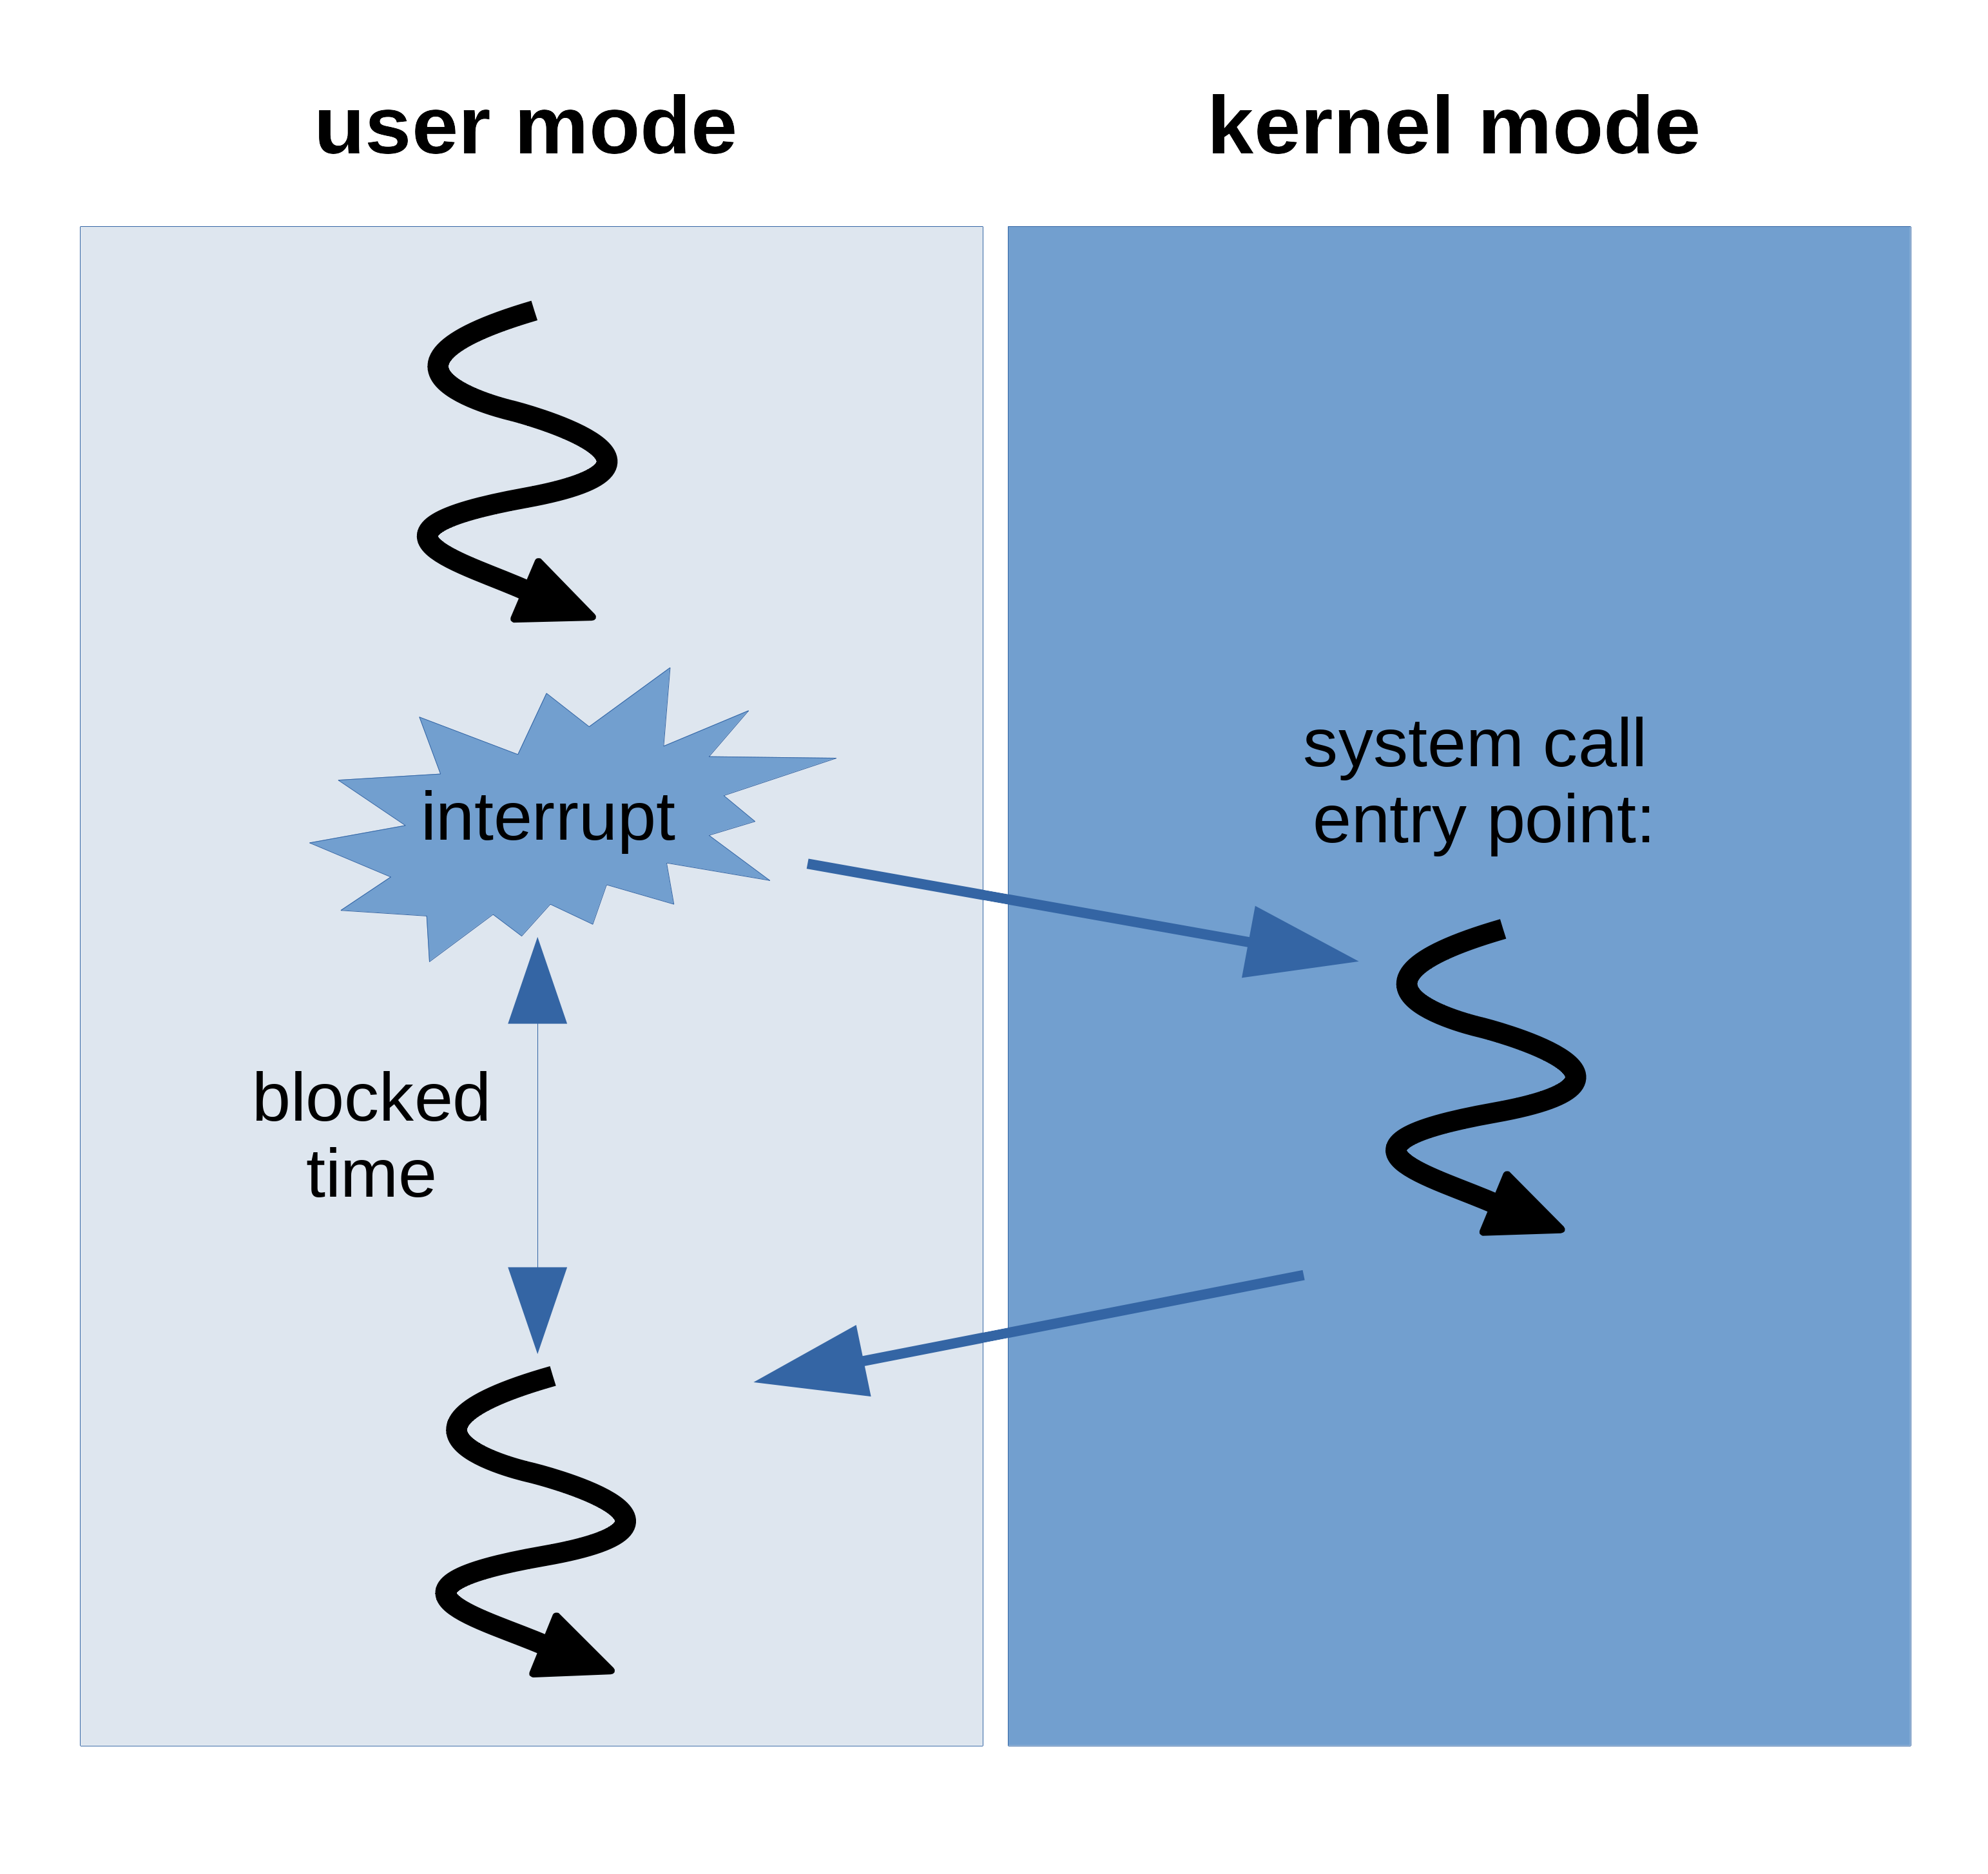
\includegraphics[scale=0.08]{syscall}
  \caption{Illustration of the CPU mode switching happening a) when the program
  generates a software interrupt and b) when the kernel completes the execution
  of a system call and returns to user-space. }
\label{fig:syscall}
\end{figure}

The way user programs voluntarily enter the kernel for system call execution is
by deliberately generating a software interrupt or exception. This is
illustrated in Figure \ref{fig:syscall}. Prior to that, the program must place
both the system call number and the system call arguments in certain CPU
registers. When the exception is generated, the CPU switches to kernel mode and
enters the kernel from a certain point which indicates that a system call has
been requested. The kernel can then examine the contents of the registers in
order to determine which system call function it needs to invoke and with which
arguments. The return value of the system call is also stored in a specific
register. When the kernel is done executing the system call, another mode
switch happens, and control returns back to the user space program.

In the x86 architecture, a user program needs to execute an \emph{INT 0x80}
instruction in order to invoke a system call in the kernel\footnotemark. This
instruction generates a software interrupt with an interrupt vector value of
0x80 which corresponds to system call exceptions. In the case of the ARM
architecture, the \emph{SVC} (formerly \emph{SWI}) instruction is used in order
to enter the \emph{Supervisor mode}.

\footnotetext{x86 additionally offers a way of performing ``fast system calls"
using the \emph{sysenter/sysexit} or \emph{syscall/sysret} pairs of
instructions which are faster than using software interrupts. The mechanics are
the same however, with the difference being that there is a separate entry
point in the kernel dedicated to system calls. This way of performing system
calls is now the standard while using a software interrupt is considered
legacy.}

\subsection{The C Library's Role}

User programs normally do not employ code that invokes system calls directly by
setting up the appropriate registers and generating an interrupt. This would be
extremely inconvenient and also non-portable. Instead, they use wrapper
functions offered by the C library which generate the appropriate assembly code
for the target architecture. The C library offers wrappers for the majority of
the available system calls plus a generic \emph{syscall} function which can be
used to easily invoke system calls for which a dedicated wrapper is not
provided.

Figure \ref{fig:libc_syscall} illustrates the steps involved in the execution
of a system call using the example of the \emph{read()} system call. The
application code calls the C library wrapper which is responsible, among other
things, for setting up the CPU registers in the way the kernel expects them and
raising an exception by using inline assembly code. The exception results in a
CPU mode switch and the invocation of the in-kernel system call handler. This
handler after examining the system call number on the appropriate register, in
turn dispatches the call to the appropriate system call service routine named
\emph{sys\_read()} in this case. Once this routine completes, execution goes
back to the system call handler which uses the \emph{iret} instruction (on x86)
in order to switch back to user mode. Control returns back to the C library
wrapper function which finally forwards the return value of the system call to
the user application.

\begin{figure}[h]
\centering
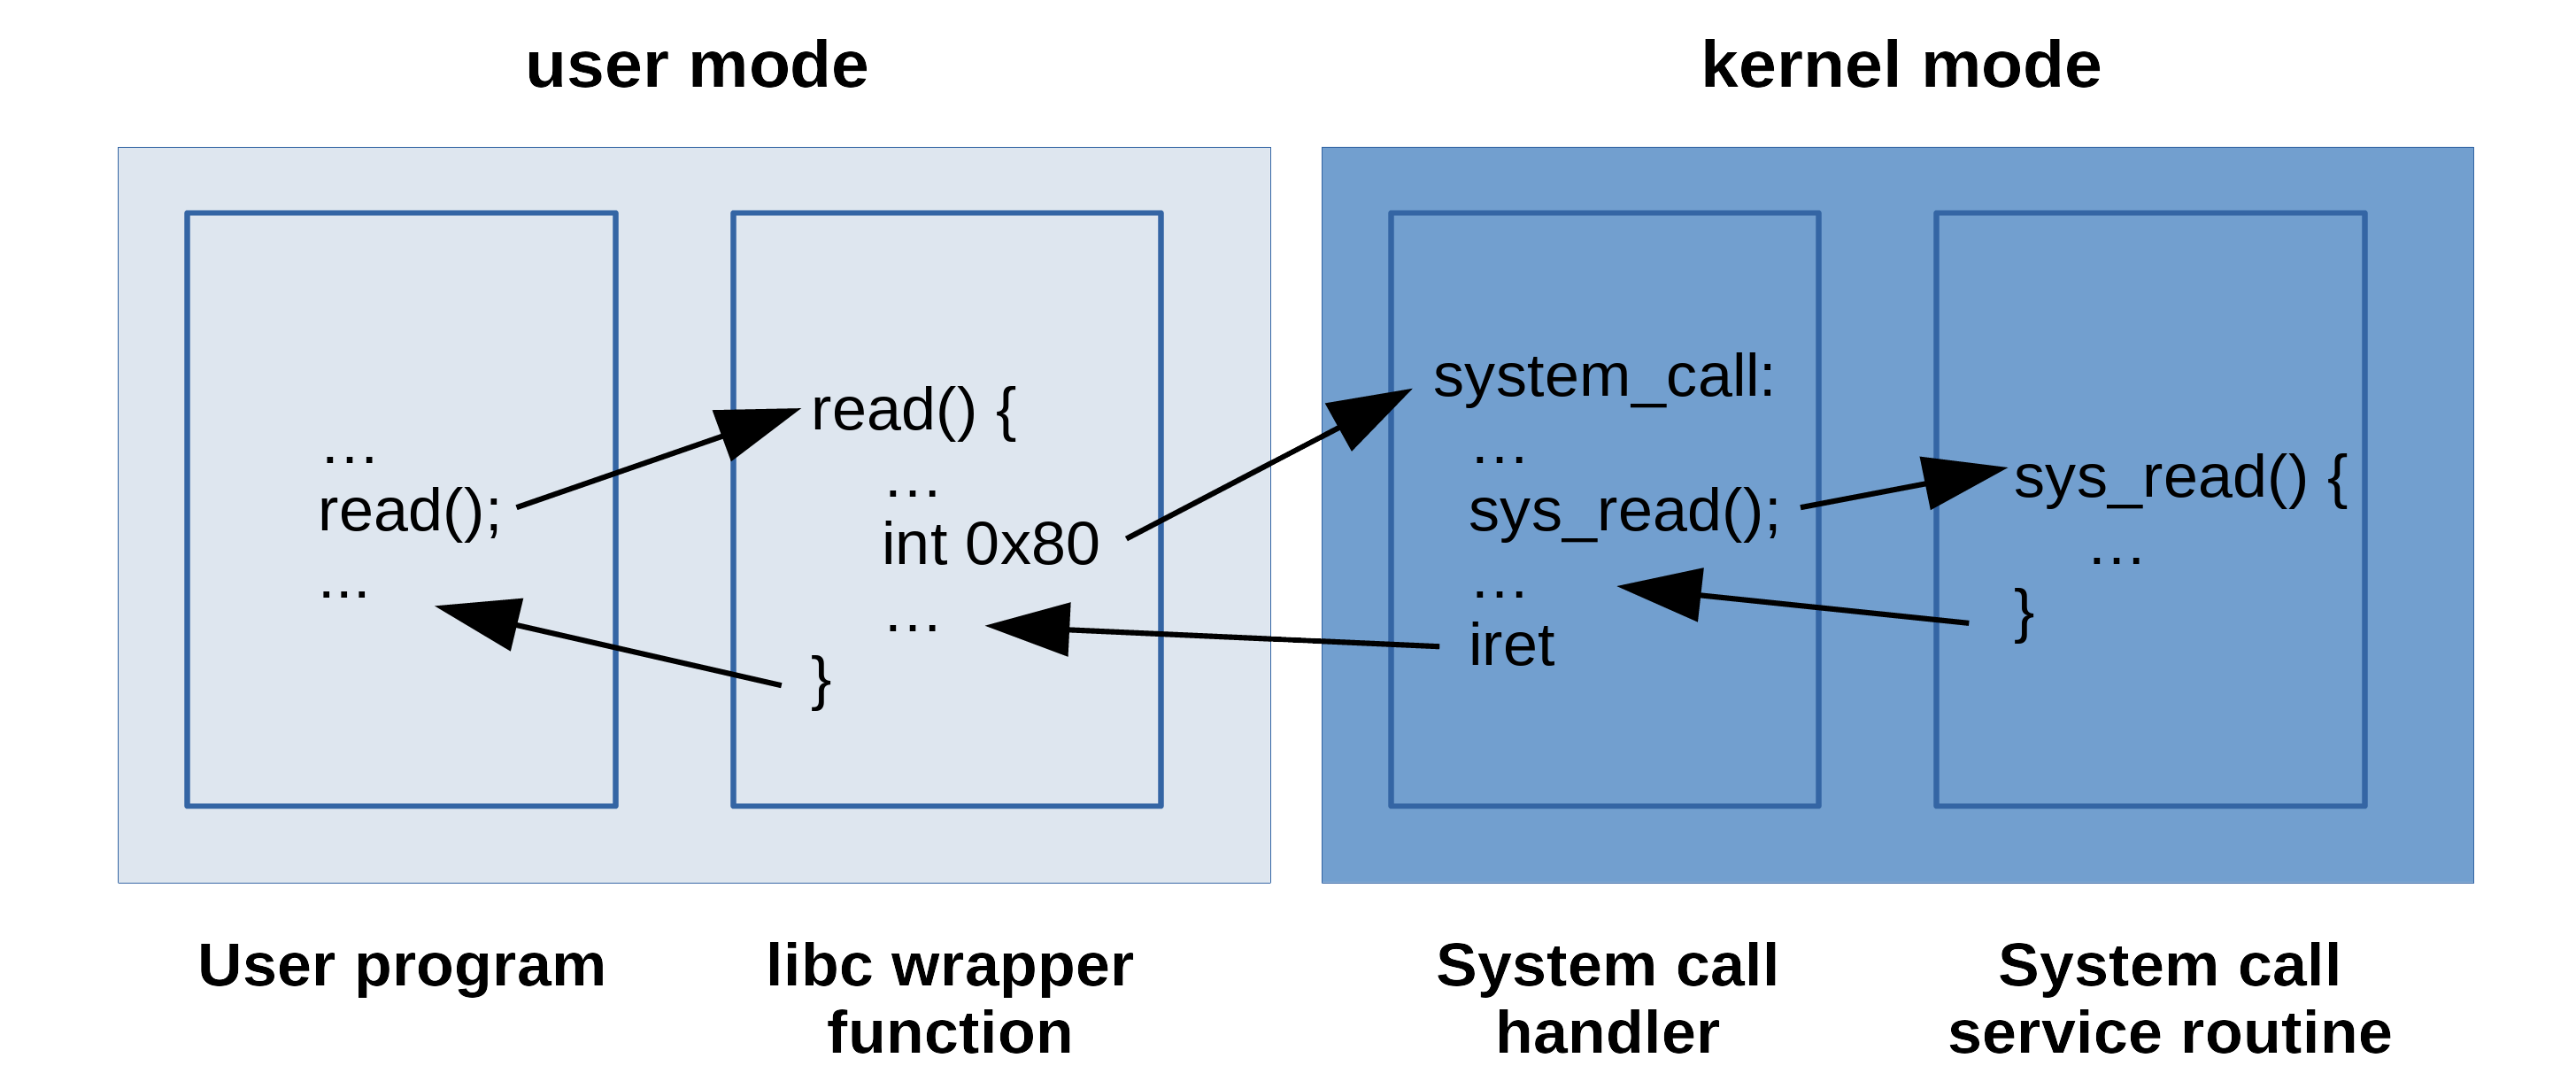
\includegraphics[scale=0.14]{libc_syscall}
\caption{Steps in the invocation of a system call using the C library}
\label{fig:libc_syscall}
\end{figure}

\subsection{System Call Invocation on Para-Virtualized \llinux}

\llinux is able to directly run unmodified Linux programs that are not aware
they are executed on a virtualized kernel. This means that these user programs
will try to invoke \llinux system calls the way they know by raising
exceptions. However, since \llinux is virtualized it does not run in a
privileged CPU mode. The kernel running in privileged mode and directly
managing the hardware is the Fiasco microkernel. That means that whenever an
\llinux task raises an exception, control will be transferred to Fiasco and not
\llinux.

Upon receipt of an interrupt, Fiasco can determine that the interrupt is
intended to be caught by \llinux since it has been generated by a vCPU thread.
In this case, it switches the address space of the vCPU to that of the \llinux
kernel. \llinux has a predefined vCPU entry point for system calls and other
asynchronous events such as page faults and hardware interrupts. Fiasco then
switches to user mode and starts executing the vCPU from that entry point.

\llinux can now see and handle the exception. When it completes execution of
the system call, it switches the address space of the vCPU to that of the
process of whose behalf it executed the system call and it lets it run on the
vCPU again. \llinux is able to switch the address space of the vCPU on its own
through a special L4 system call.

\subsection{System Call Invocation from Decoupled Threads}
\label{sec:syscall_forwarding}

Decoupled L4 threads run on a possibly isolated core, managed by Fiasco, on
which no vCPU is executing. That means that when a detached L4 thread wants to
invoke an \llinux system call, the execution of the system call needs to happen
on a different CPU core on which \llinux is running (inside a vCPU).

In this case, system calls are essentially forwarded to some CPU hosting
\llinux. The mechanics are similar to the one described in the previous section
but this time cross-processor communication is required. Again, when the
decoupled thread generates an exception, it traps into Fiasco which in this
case creates an L4 IPC message.

This IPC message appears to come from the faulty thread and is directed to its
exception handler which is the vCPU hosting the corresponding kernel-side
context. Since the sender and receiver are in different cores, cross-core IPC
is used which is significantly slower than core-local IPC. The reason it's
slower is that it uses inter-processor interrupts as its notification mechanism
in order to interrupt the execution of the remote processor.

When the interrupt hits the other processor, the Fiasco kernel running there
forwards the exception to the appropriate vCPU. Once \llinux receives the
exception (i.e. the IPC message), it wakes up the corresponding kernel-side
context of the decoupled thread described in section \ref{sec:decoupling}. This
thread, whose only purpose is to run \llinux kernel code handling exceptions on
behalf of the decoupled thread, finally executes the system call. After
completing the system call execution, \llinux puts this thread back to sleep
and it doesn't wake it up until there is a new exception that it needs to
handle for the decoupled thread.

Once the return value of the system call is ready, \llinux needs to inform the
core hosting the decoupled thread by replying to the original IPC message. At
this point, another inter-processor interrupt needs to be used for signaling.
This cross-processor forwarding using inter-processor interrupts comes with a
significant performance overhead over both native Linux and \llinux without
decoupling. This can be prohibitive for time-critical or frequently used
operations. It becomes clear that the L4 architecture needs a faster way of
forwarding system calls from decoupled threads to \llinux.

\section{Virtual System Calls and the vDSO}

As explained in the previous sections, executing a system call requires at
least one CPU mode switch. However, a few simple system calls that merely
return information form the kernel are trivial enough that they can be executed
without requiring a transition to kernel mode. That's why the Linux virtual
Dynamic Shared Object (vDSO) \cite{vdso} was created.

The Linux vDSO is a small shared library containing kernel code which the
kernel maps into the user space part of the address space of all applications.
Some simple frequently used system calls such as \emph{gettimeofday} can then
be executed without entering the kernel at all. Only read-only system calls
qualify for this since user-space processes are not allowed to write into the
kernel address space.

Due to the address space layout randomization (ASLR) security mitigation that
is enabled in most systems, the location of vDSO is not fixed. The C library
takes care of the task of locating the vDSO object in runtime by looking for an
auxiliary ELF header in which the kernel writes its address when the program is
loaded. The C library then uses the vDSO whenever possible and the whole
process is transparent to applications.

The vDSO mechanism is supported in \llinux in both decoupled and no-decoupled
mode \cite{decoupling}. That means that when a detached thread issues a
vDSO-supported system call, no cross-processor communication is required.
Nevertheless, the amount of system calls included in the vDSO is quite small.
This depends on the architecture, but for example, on x86\_64 only 4 system
calls are supported; \emph{clock\_gettime}, \emph{clock\_getcpu},
\emph{get\_timeofday}, and \emph{time}. Other architectures support more, but
usually not more than 10.

Therefore, vDSO system calls alone are not enough to compensate for the extra
performance overhead the decoupling mechanism introduces. Most applications
will use a large variety of system calls, most of which not included in vDSO.

\section{System Call Batching}

Previous studies have highlighted the performance gains when using system call
batching techniques
\cite{clustering}\cite{compositecalls}\cite{cassyopia}\cite{compositecalls2}.
Crossing the user-kernel boundary often can have significant overhead in terms
of performance for reasons of mode switching and cache pollution.

Normally, when a user process issues a system call, the user mode pipeline is
flushed, the privilege level of the CPU changes, and kernel code starts
executing. Execution of kernel code results in the pollution of system caches.
Once the kernel is done executing a system call, another mode switch happens
and user code of the application starts executing again, but this time causing
many more cache misses since the data and instruction caches have been filled
with kernel data. These cache misses can affect performance significantly.
Specifically, it can take up to 14,000 cycles of execution before the
instructions per cycle rate of the application returns to the same level as
before executing a system call \cite{flexsc}.

The idea behind system call batching is that user programs can collect a number
of system calls before they ask the kernel to execute them all at once. This
way the system call related overhead is minimized since now only two CPU mode
switches are required for executing each batch. The cache pollution because of
the kernel execution also happens much less frequently.

One drawback is that existing applications need to be modified in some way in
order to use system call batching techniques. Also, most operating systems do
not inherently offer such a mechanism. Additionally, system call batching might
not be feasible for some applications or algorithms at all. Many programs
cannot issue further system calls or otherwise make progress before previously
issued system calls complete. Nevertheless, new applications if written in a
way that allows batching of system calls, and by using the appropriate
libraries or tools, they can observe significant performance gains.

\section{Exception-Less System Calls}

A 2010 paper from Livio Soares and Michael Stumm has introduced the concept of
exception-less system calls and a Linux implementation of it called FlexSC
\cite{flexsc}. Using the FlexSC mechanism user applications can post system
calls in memory, instead of using the traditional scheme with software
exceptions and arguments passing via CPU registers. The Linux kernel then picks
them up from there in order to execute them and writes the return value back to
the shared memory area.

FlexSC is focused on highly threaded applications. The main idea is that
different threads of the same process can post system calls in memory, one
each. Once a thread posts a system call it goes to sleep and another thread of
the same application gets user-level scheduled. All these threads could not
execute in parallel anyway, since there is the limit of the physical CPU cores
available in the system. When some or all of the threads have posted a system
call and therefore cannot proceed, a traditional exception-based system call is
used to indicate to the kernel that it needs to start processing the system
calls that have already been posted to memory for this process.

This scheme allows for batching system calls, but instead of the applications
having to prepare the batches themselves, the batches are automatically created
from system calls of different threads that share the same address space.  For
this purpose, the authors of the paper have developed a user-space threading
library compliant with POSIX Threads and binary compatible with NPTL, the
default thread library on Linux. The difference is that the threads are managed
and scheduled by the library itself in user-space as in a green threads model.
This library allows existing applications to transparently use the
exception-less system calls mechanism without requiring modifications to their
source code or recompilation.

While FlexSC seems to notably improve the performance of heavily multi-threaded
applications with hundreds or thousands of threads, it does not seem to provide
any performance benefits to existing single-threaded applications or
multi-threaded applications that use a small number of threads. Nevertheless,
the idea of invoking system calls using shared memory and without using
software interrupts (which are a major bottleneck for decoupled threads as
described previously), served as an inspiration for the creation of a faster
system call forwarding mechanism for \llinux.
